\begin{refsection}
In this chapter, all the important choices for the models setup are reviewed and discussed. The motivation for
these choices comes from the literature review of the numerical modelling aspects from the previous section
and also from some information coming from the appendix. The goal of these experiments are to describe the flow and transport characteristics that can be used in a further step to determine the influence of vegetation. The experiments cover flow visualisations, velocity and concentration measurements. Both quantitative and qualitative properties were used to describe the nature of the flow.

\section{Flow Profiling}
In this section, the method used to set-up a model to describe a simple open channel flow case. This case was later used as sampled profile for the main simulation.
\subsection{Flow Conditions}
\label{sec:flowConditions}
A summary of the hydraulic parameters is presented in table \ref{tab:inlet}. The height(\textit{H}) of the domain, mean channel velocity (\textit{U}) and Reynolds number (\textit{Re}) are selected to be the same with the experiment of \textcite{xiang2019}.
\begin{table}[]
\centering
\caption{Hydraulic conditions for the development of the flow.}
\label{tab:inlet}
\begin{tabular}{lllll}
Geometry     & H(m) & U(m/s) & Re(-) & Fr(-) \\ \hline
Main Channel & 0.1  & 0.101  & 9000  & 0.102
\end{tabular}
\end{table}

\subsection{Grid and Boundary Conditions}
A simple 3D rectangular channel was built. The model consisted of a single rectangular box with length of 0.25 m in the stream-wise direction (\textit{x-axis}), 0.30 m in the span-wise direction (\textit{y-axis}) and 0.10 m of depth (\textit{z-axis}). Excluding the stream-wise direction, the geometry follows the experimental main channel conditions.

The mesh tailored for this domain was divided into a regular grid composed of hexahedrons with $\Delta_x =75$, $\Delta_y = 240$ and $\Delta_z = 90$. The divisions were homogeneous in the \textit{x-axis} and was graded in the other directions. The grading allowed the mesh to be sufficient fine at near wall zones, providing a better resolution of the flow. The turbulent properties of the channel were calculated based on the typical channel flow presented in \textcite{Pope2000}. The implemented procedure allowed to estimate the scales of the flow serving as a comparison to the numerical results and it is comprised in the the python script bellow.

\begin{lstlisting}[language=python]
B = float(input("Channel width (B): "))
H = float(input("Flow depth (h): "))
U = float(input("Mean velocity (U): "))
Re = float(input("Reynolds number: "))
yplus = float(input("Desired y+: "))

#Reynolds Number Near the Wall
Ret = 0.09*Re**(0.88)
print("Near Wall Reynolds Number:",Ret)

#Viscous Lengthscale
deltaV = H/Ret
print("Viscous Lengthscale:",deltaV,"m")

deltayplus = deltaV*yplus
print("Distance to desired y+:",deltayplus,"m")

#Friction Velocity
Ut = 1e-6/deltaV
print("Friction Velocity (Velocity Scale):", Ut,"m/s")

#Turbulence Lengthscale
Lt = 0.07*B
print("Turbulence Lengthscale:",Lt,"m")

#Turbulence Intensity
It = 0.16*Re**(-1/8)
print("Turbulence Intensity:",It)

#Turbulent Kinectic Intensity
k = 1.5*(U*It*100)**2
print("Turbulent Kinectic Intensity:",k,"m2/s2")

#Turbulent Dissipation Rate
E = ((0.09**0.75)*(k**1.5))/Lt
print("Turbulent Dissipation Rate:",E,"m2/s2")

#Turbulent Specific Dissipation Rate
W = (k**0.5)/((0.09**0.25)*Lt)
print("Turbulent Specific Dissipation Rate:",W,"1/s")

#Mixing Length
hydDiameter = 4*(H*B)/(2*H+B)
ML = 0.07*hydDiameter
print("Mixing Length:",ML,"m")

f = open("results.txt","w+")
f.write("Near Wall Reynolds Number: {:.2f}\n".format(Ret))
f.write("Viscous Lengthscale: {:.2e} m\n".format(deltaV))
f.write("Desired y+: {:.2f}\n".format(yplus))
f.write("Distance to desired y+: {:.2e} m\n".format(deltayplus))
f.write("Friction Velocity (Velocity Scale): {:.2e} m/s\n".format(Ut))
f.write("Turbulence Lengthscale: {:.2e} m\n".format(Lt))
f.write("Turbulence Intensity: {:.1%}\n".format(It))
f.write("Turbulent Kinectic Intensity: {:.2f} m2/s2\n".format(k))
f.write("Turbulent Dissipation Rate: {:.2f} m2/s2\n".format(E))
f.write("Turbulent Specific Dissipation Rate: {:.2f} 1/s\n".format(W))
f.write("Mixing Length: {:.2e} m\n".format(ML))
f.close()
\end{lstlisting}

The turbulent length scale was calculated using the simplification that in open channel flows the scales is 7\% of the channel width (Line 44). As the numerical domain is slightly shorter than the experimental channel (experimental = 0.85 m) the experimental width was used in the procedure, resulting in $L_T = 0,0595$ m. The calculated mixing layer near to the wall was 7.21e-03 m and the viscous lengthscale was $\delta_v=1.06e-04$ m. Once the pre-setup variables were calculated the boundary conditions were then chosen to best develop the flow in the channel.

The development of the turbulent flow was performed by a \textit{pseudo-cyclic} condition in both inlet and outlet surfaces, for velocity and pressure, the mapped function. The mapped BC implies that a pressure gradient or a mean velocity must be given at the domain in order to drive the flow. Here the mean velocity approach was chosen and was defined in equation \ref{eqn:mappedVel}. This condition is called \textit{pseudo-cyclic} because the cells at the inlet surface can not alter the outlet cells as a traditional cyclic boundary condition would, instead the changes from the inlet to the previous outlet are considered as a zero gradient. 
\begin{equation}
U=\frac{1}{h}\int_{0}^{h}<u>dz
\label{eqn:mappedVel}
\end{equation}
This is added into the model as an average condition to the variable value (ie.  velocity, pressure,...), as example the velocity boundary condition at the coupled surfaces:

\begin{lstlisting}
inlet
{
	type            mapped;
	field           U;
	setAverage      true;
	average         (0.101 0 0);
	interpolationScheme cell;
	value           uniform (0.101 0 0);
}
outlet
{
	type			zeroGradient;
}
\end{lstlisting}

The slip boundary condition (BC) was applied to the top boundary (z = 0.1 m), this representation of the atmosphere (rigid-lid approximation) is allowable when the Froude number (\textit{Fr}) is lower than 0.5 \cite{alfrink1983}. As the physical domain extends further than one cavity width in the \textit{y-axis} it was possible to cut the channel in order to save computational time \cite{Brevis2014}. The surface plane that contains this cut is at y=0 and it was also represented as a slip BC. The no-slip BC was applied to the other surfaces. Once the boundary conditions were satisfied, a proper choosing of numerics and models was required.

The turbulence properties were calculated using a Reynolds-Averaged Navier-Stokes (RANS) approach. The chosen model was the $ k-\omega$ SST due to a higher precision near the wall compared to traditional $k-\epsilon$ and a faster and more accurate resolution at far-wall regions compared to $k-\omega$. The simulation ran in a permanent solution using the Semi-Implicit Method for Pressure-Linked Equations (SIMPLE), under the package simpleFoam.

In order to verify the simulation results  the values were compared to the calculated parameters from Pope's procedure. The numerical model proposed to develop the flow could find close values to calculated ones. The velocity profile in the free surface was qualitatively equal to the traditional turbulent wall bounded open channel case (Figures \ref{fig:flowProfVel} and \ref{fig:flowProfVelChart}). The velocity remained to its maximum near $y=0$, where the slip wall BC was implemented region closer to the middle of the channel ($X=0.425$ m), while a sharp gradient occurs at $y=0.30$ m region where the no-slip wall was set. The Reynolds stress tensor was calculated for all domain and had its peak at the highest velocity magnitudes as expected (Figure \ref{fig:flowProfReyStress}).

\begin{figure}[!ht]
  \centering
  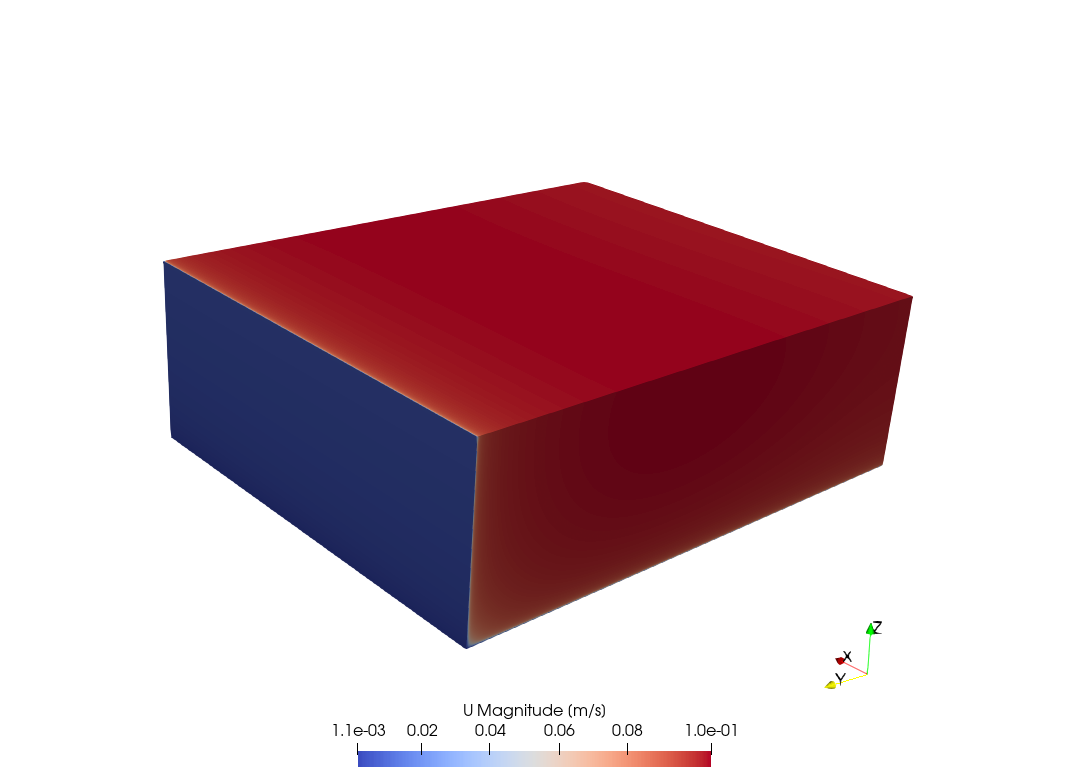
\includegraphics[width=\linewidth]{../images/methods/flowProfVelocity.png}
  \caption{Velocity contour of the flow profiling simulation.}
  \label{fig:flowProfVel}
\end{figure}
\begin{figure}[!ht]
  \centering
  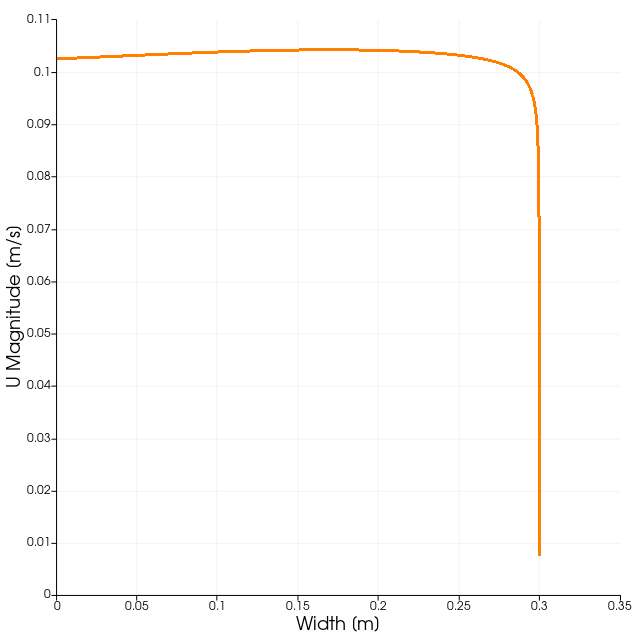
\includegraphics[width=0.5\linewidth]{../images/methods/flowProfVelocityChart.png}
  \caption{Velocity profile in the \textit{y-axis}, in $z=h$}
  \label{fig:flowProfVelChart}
\end{figure}
\begin{figure}[!ht]
  \centering
  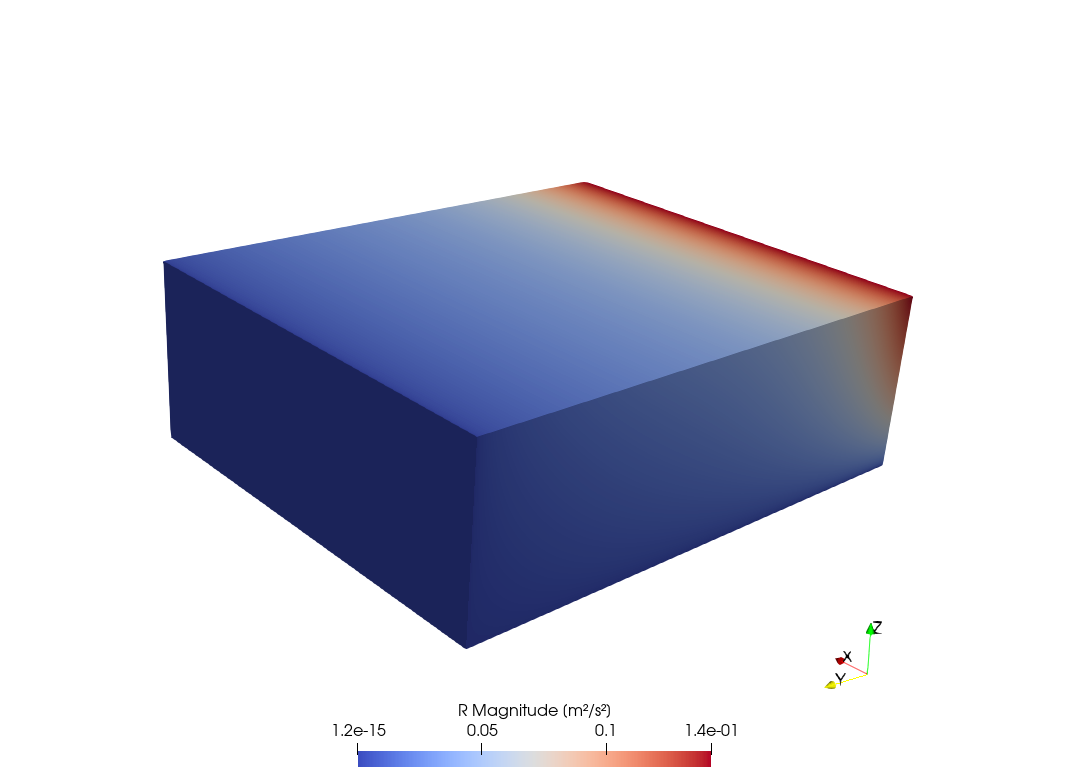
\includegraphics[width=\linewidth]{../images/methods/flowProfReynoldsStress.png}
  \caption{Reynolds stress tensor magnitude contour of the flow profiling simulation.}
  \label{fig:flowProfReyStress}
\end{figure}

Once the results were compared, the outlet surface was then sampled for velocity, pressure, Reynolds stress tensor and turbulence intensity. Those information were later used in the main simulations as the inlet. Since the flow is already developed, this inlet approach saved computational resources, by reducing the inlet portion of the channel, allowing a mesh refinement in needed regions (eg. cavity interface, near-wall regions, etc).

\section{Large Eddy Simulation (LES)}
In this section, the numerical model is described in detail.

\subsection{Geometry and Mesh}
The geometry was set to describe the experiments of \textcite{xiang2019}. The experiment consisted in a single lateral cavity adjacent to a rectangular open channel (Figure \ref{fig:geometry}). The lateral cavity was $L = 0.15$ m wide and $W = 0.25$ m long, consisting in an aspect ratio of $W/L = 0.6$, what corresponds to a single circulation flow inside the cavity. The flow conditions of the main channel were pre-calculated and described in the earlier section.

\begin{figure}[!ht]
  \centering
  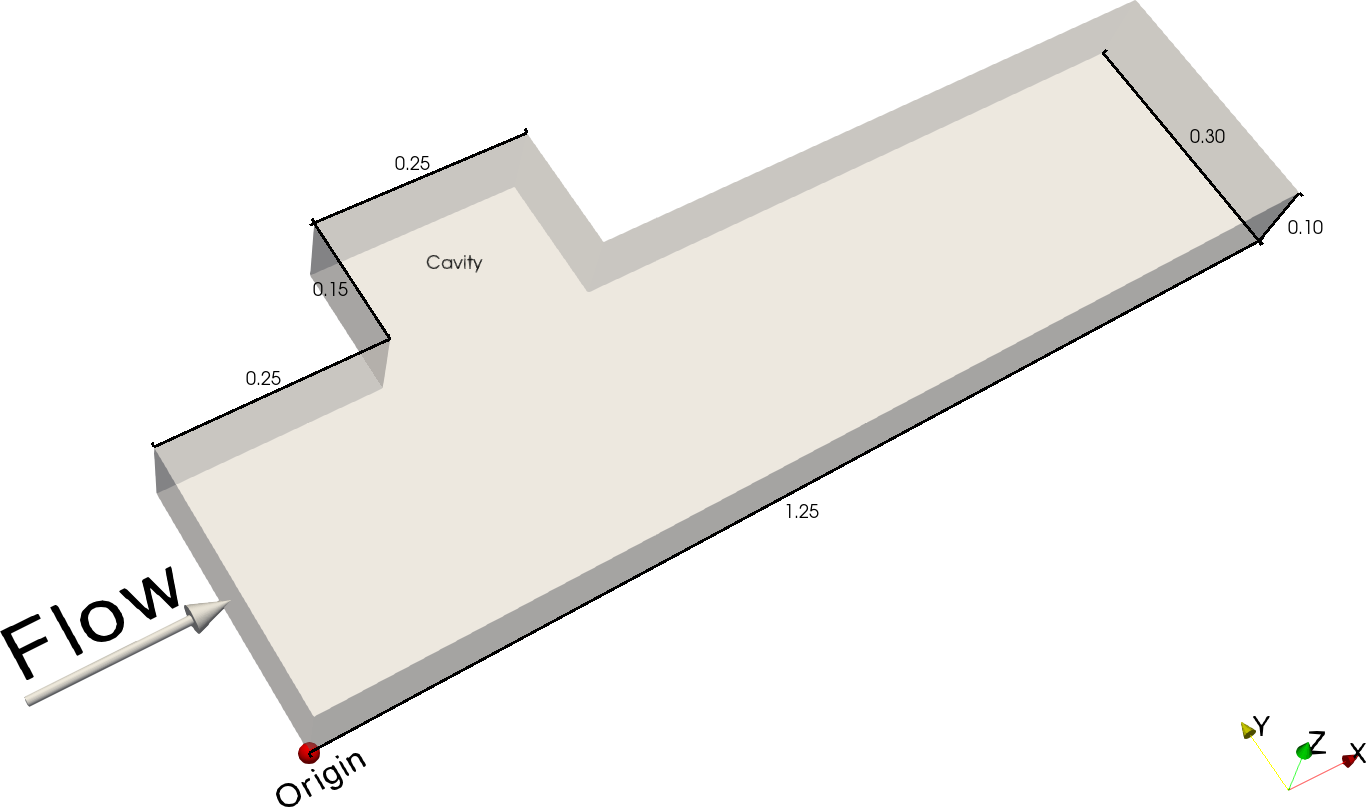
\includegraphics[width=\linewidth]{../images/methods/geometry.png}
  \caption{Computational domain with coordinates and dimensions.}
  \label{fig:geometry}
\end{figure}

The mesh was calculated in an structured approach for a faster implementation of the model.  Similarly to flow profiling simulation, the domain was divided homogeneously in the \textit{z-axis} and was graded at near-wall regions for a better resolution of the flow at these scales, being the maximum value of $y^{+}=5$ that is a region within the viscous sub-layer. The adopted distance at near-wall is the maximum value recommended for a LES simulation and for this reason a wall model was implemented and will be further detailed in section \ref{sec:BC}, after the mesh is discussed and set in the following sections.

\subsection{Grid Convergence Index (GCI)}
In order to estimate the influence of grid errors in the model, a GCI test was implemented. This approach is based on the procedure created by \textcite{celik2008}. The initial mesh (mesh 3) was composed of hexahedrons with $\Delta_x =68$, $\Delta_y = 68$ and $\Delta_z = 20$ in the lateral cavity volume. The rate of growth of the cells was maintained in 1 in the \textit{x-axis}, 2 in the \textit{y-axis} and 41 in the \textit{z-axis}. The first mesh (mesh 3) totals 639,680 elements. As the procedure advises a change in 30\% of the representative grid size $h$ (Equation \ref{eqn:hGCI}),  all the three meshes adopted for the GCI analysis are summarised in the table \ref{tab:gci}.
\begin{equation}
h=\left [\frac{1}{N}\sum_{i=1}^{N}(\Delta V  _i)\right ]^{1/3}
\label{eqn:hGCI}
\end{equation}
where N is the number of cells, $\Delta V_i$ is the volume of the cell.

\begin{table}[]
\centering
\caption{Summary of all meshes adopted in the Grid Convergence Index (GCI) analysis. $\Delta_i$ values corresponds to the number of divisions inside the lateral cavity.}
\label{tab:gci}
\begin{tabular}{llllrrlr}
Mesh & $\Delta_x$ & $\Delta_y$ & $\Delta_z$ & \multicolumn{1}{l}{Number of Elements} & \multicolumn{1}{l}{h} & \multicolumn{2}{l}{Refinement Rate} \\ \hline
1    & 100        & 100     & 44         & 3,132,800                              & 0.0214                & $R_{21}$   & 1.293                  \\
2    & 80         & 80         & 40         & 1,408,000                              & 0.0277                & $R_{32}$   & 1.294                  \\
3    & 68         & 68         & 20         & 639,680                                & 0.0359                &            & \multicolumn{1}{l}{}  
\end{tabular}
\end{table}

Onde all the three meshes were calculated, the results needed to be compared and a main variable chosen to capture the influence of meshing in the solution. As the flow inside the cavity is the main focus of this dissertation, the variable chosen for this test was the time averaged velocity in the streamwise direction inside the embayment. The extraction of this variable adopted a sampling of a surface at $z/h = 0.6$, the planar results were later condensed by a ensemble averaged procedure that allowed the data to be visualised in a 2D chart. The results of the three grid are presented in Figure \ref{fig:gciAllMeshes}.
\begin{figure}[!h]
\centering
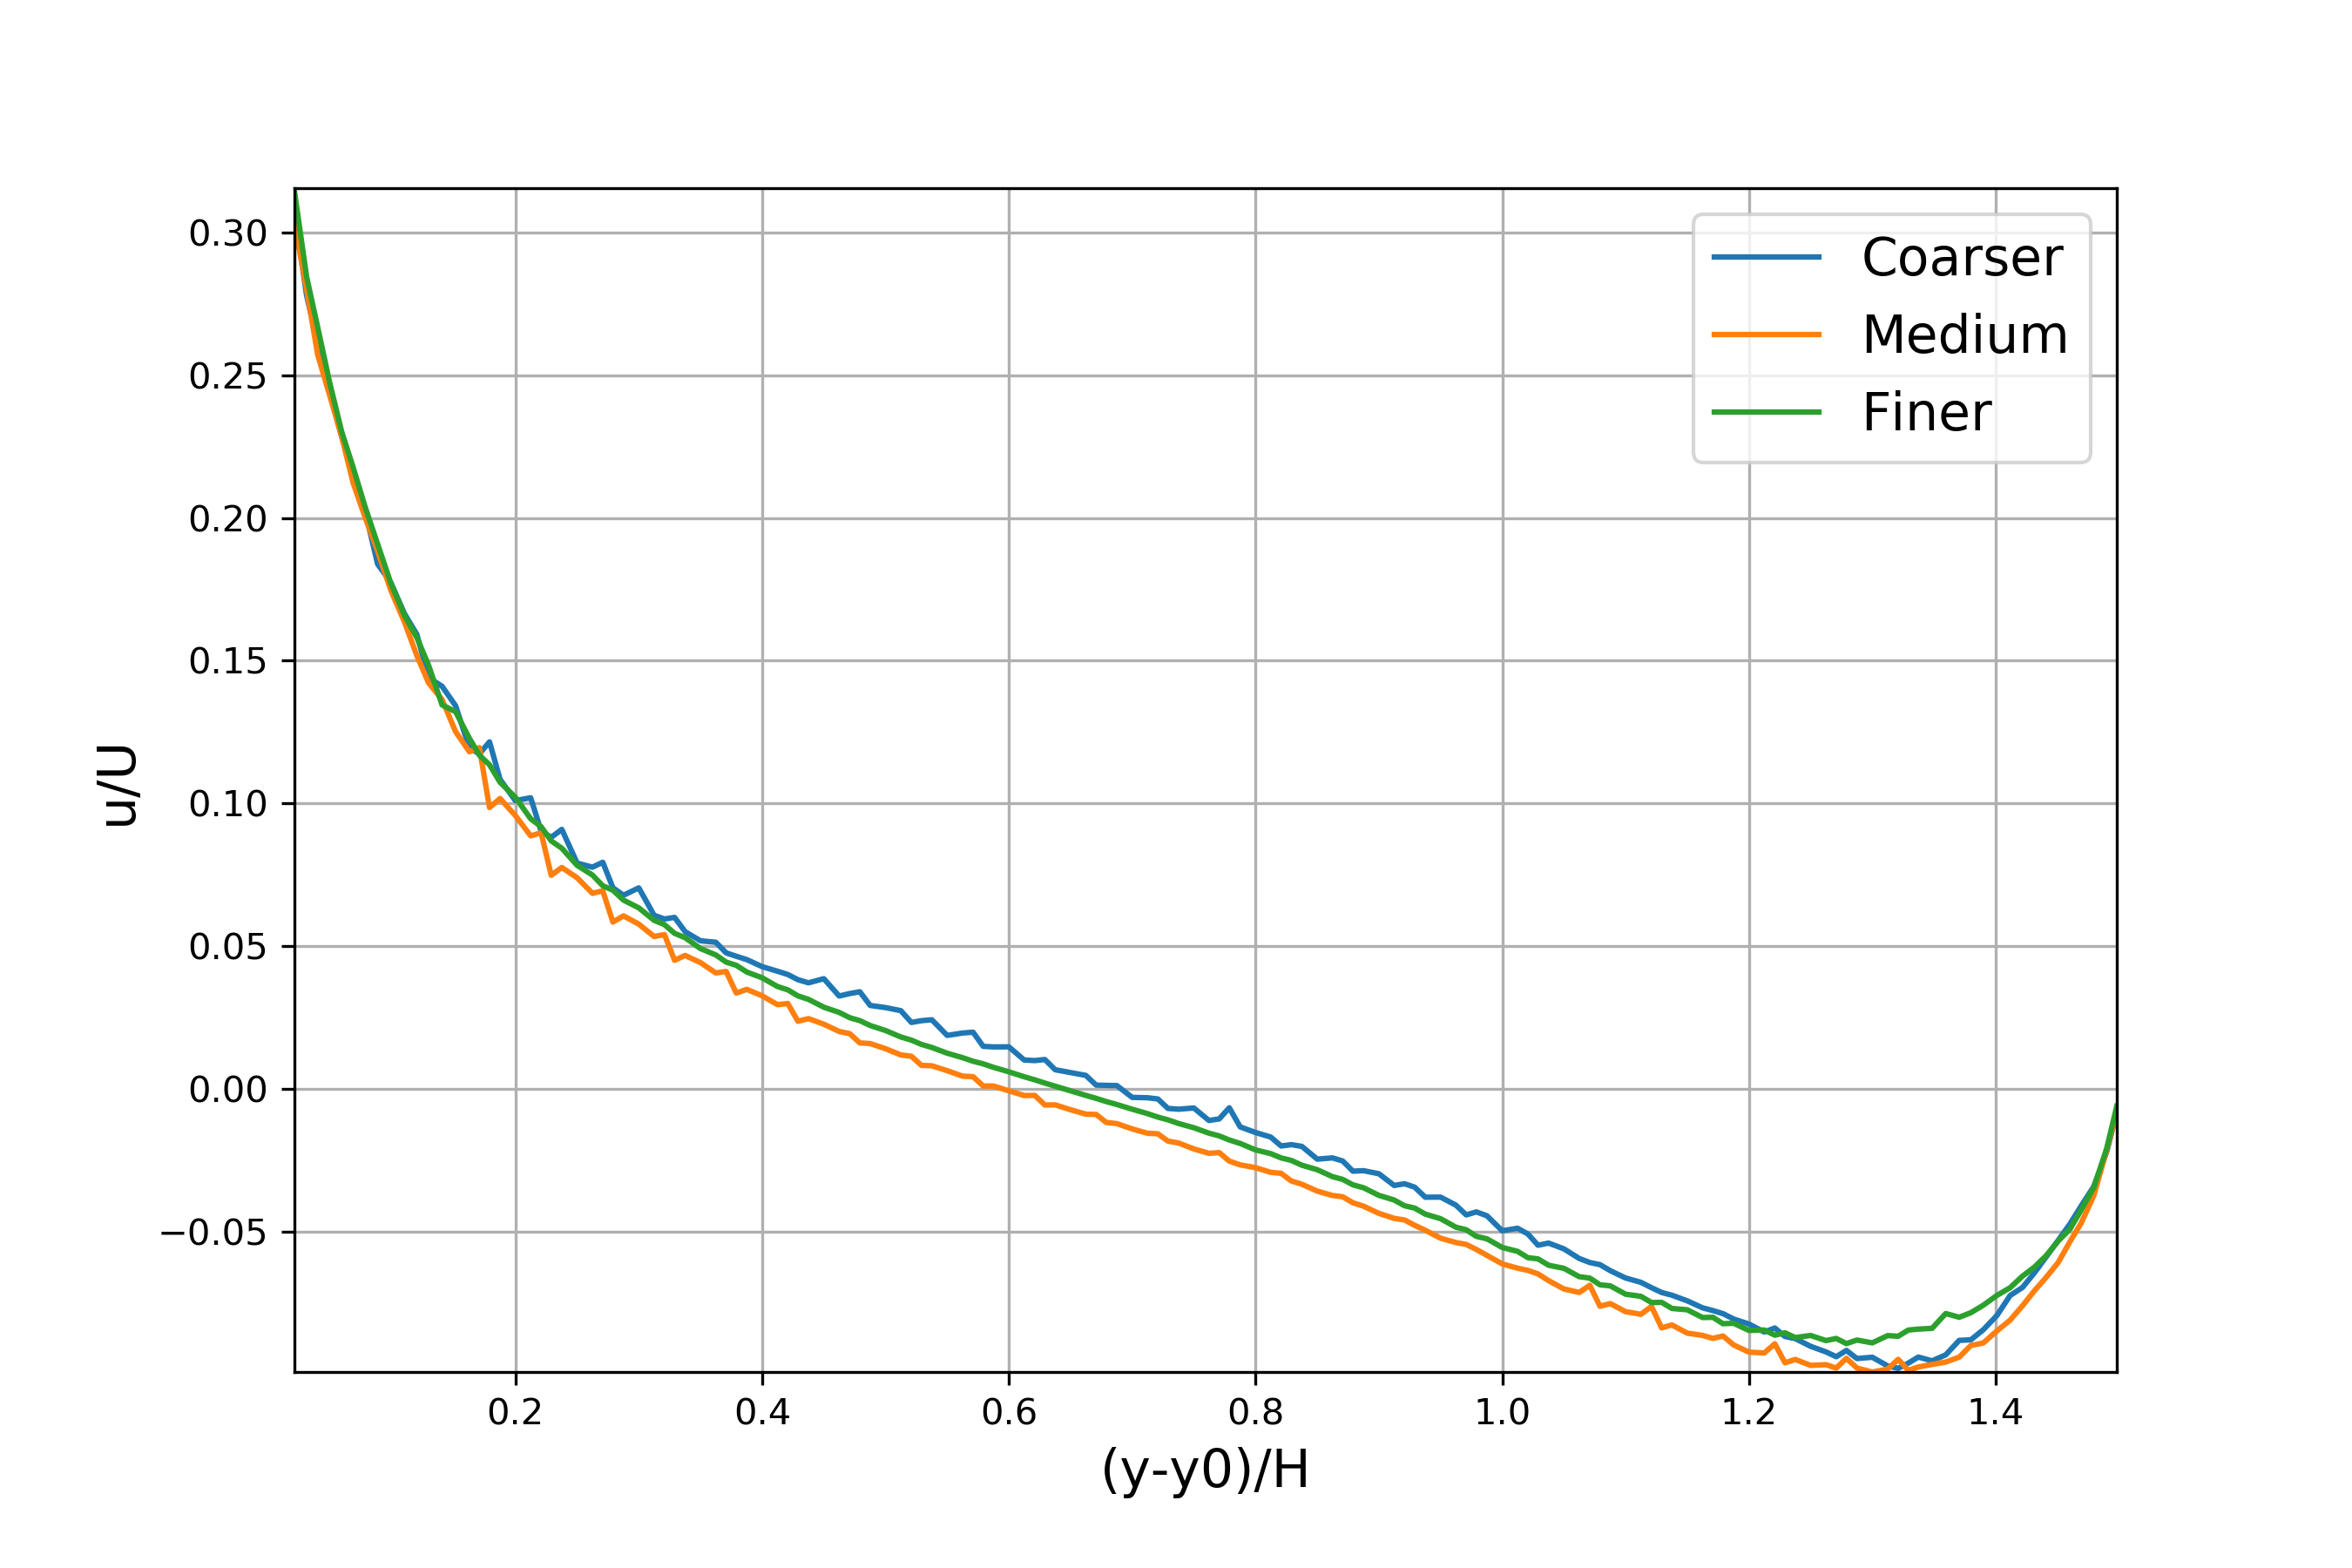
\includegraphics[width=\linewidth]{../images/methods/gciAllMeshes.png}
\caption{Comparison of the time ensemble averaged velocity inside the lateral cavity.}
\label{fig:gciAllMeshes}
\end{figure}

The GCI analysis concluded in a oscillatory convergence around the experimental data. This indicates two possible scenarios: adopt the mesh with better agreement (mesh 2) or further refine the mesh in order to minimise the oscillation. As a further refinement would require more computational time the mesh 2 was chosen. The expected error in mesh 2 is described in Figure \ref{fig:gciErrorbar}, the maximum values of error occurred in high velocity gradient regions ($0<(y-y_0)/H<0.2$), this implies that further refinement would be preferable in this regions, especially in the mixing layer since all the energy of the flow comes from this region ($0<(y-y_0)/H<0.2$).
\begin{figure}[!ht]
\centering
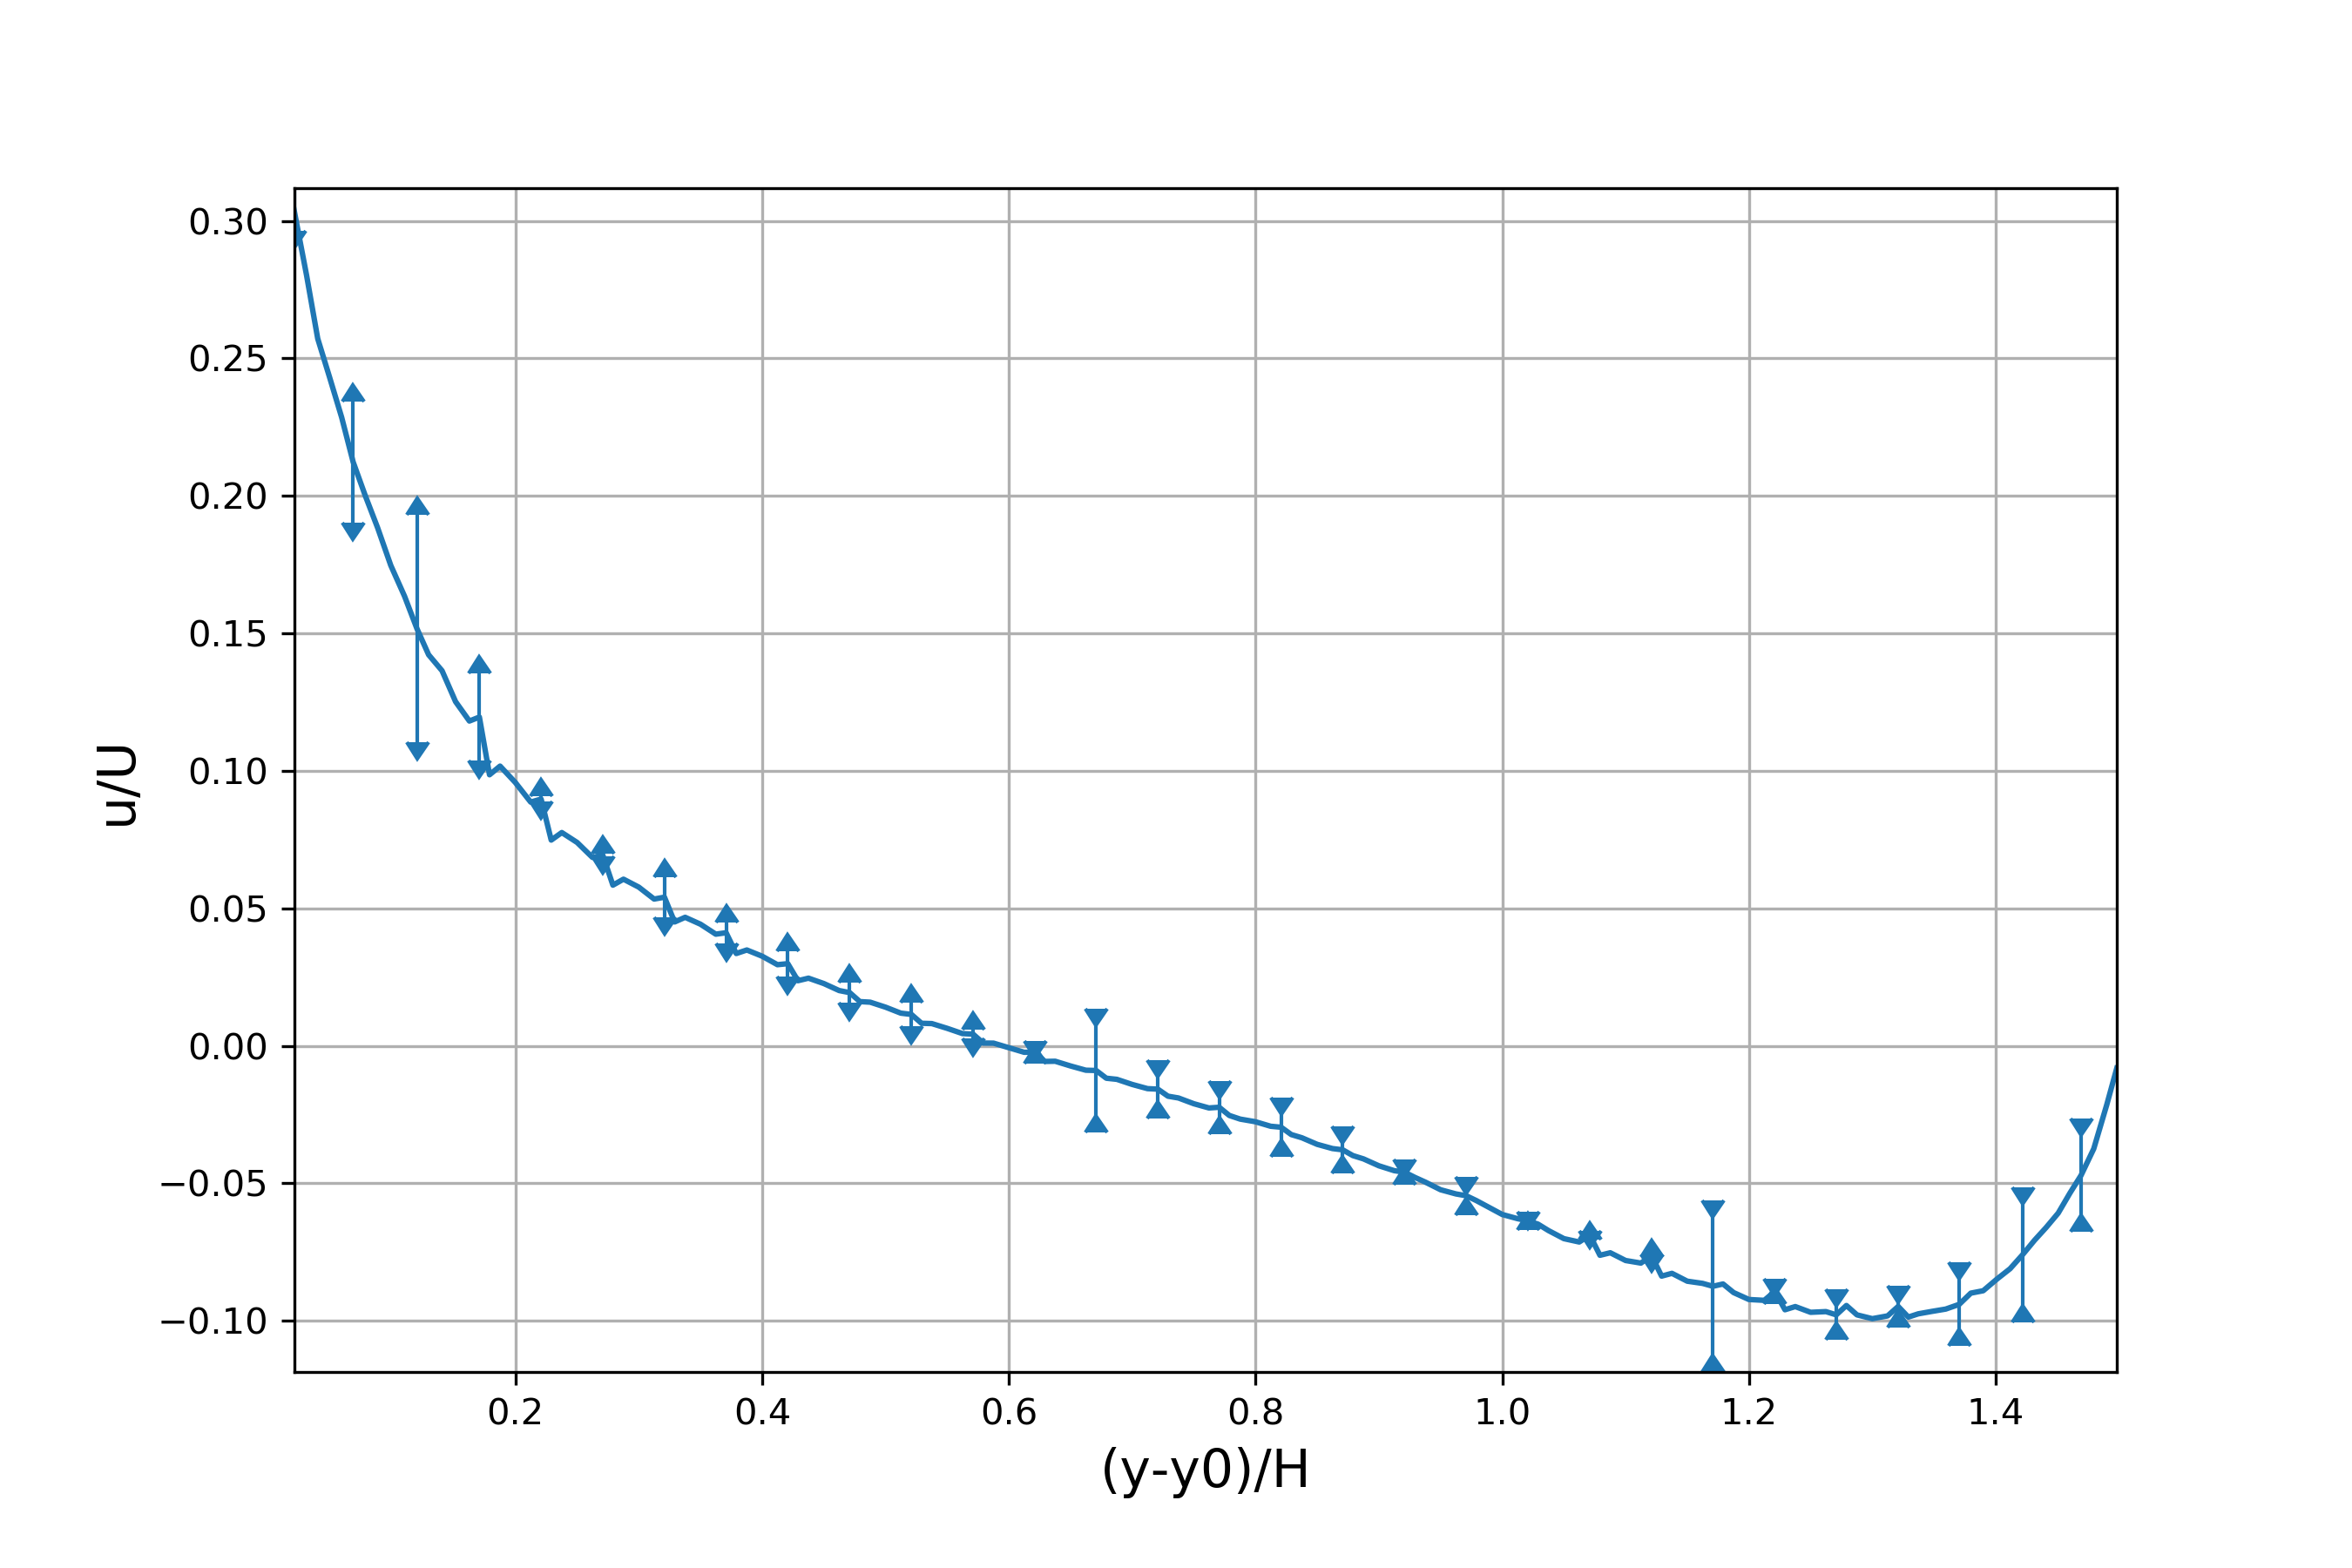
\includegraphics[width=\linewidth]{../images/methods/gciMediumWithErrorbars.png}
\caption{Ensemble averaged streamwise velocity ($u$) with error bars.}
\label{fig:gciErrorbar}
\end{figure}

The implementation of this procedure was realised by a python script published by myself under the public repository on \href{https://github.com/Worth-Option/gci}{GitHub} and can also be found in the Appendix \autoref{chap:appendixA}.

\subsection{Turbulence Modelling}
Once the meshing was discussed, the physical models are now disclosed in this subsection.

The turbulence was calculated using a wall modelled LES. The sub-grid model determines the sub-grid scale viscosity in the near wall region. This implies that the simulation is partially modelled for events smaller than the grid and resolved for larger eddies \cite{versteeg2007}. The LES equations uses the idea of spatial filtering to separate the larger and smaller eddies. The filtering function used was the cubic root volume that is defined in equation \ref{eqn:filterLES}.
\begin{equation}
\Delta = c \left( V_c \right)^{\frac{1}{3}}
\label{eqn:filterLES}
\end{equation}
where $c$ is a model coefficient defined as 1, and $V_c$ is the volume of the computational cell. This filter was used since the chosen sub-grid model does not require a damping function, otherwise the van-Driest function should be implemented.
In this section the over-bar indicates spatial filtering, not time-averaging. As the investigated flow is incompressible, the Navier-Stokes equations (NS) are simplified and its filtered version is defined as:
\begin{equation}
\frac{\partial \overline{u_i}}{\partial t}+\frac{\partial }{\partial x_j} \left ( \overline{u_i u_j} \right )= -\frac{1}{\rho}\frac{\partial \overline{p}}{\partial x_i}+\frac{\partial }{\partial x_j} \left [ \nu \left ( 2 \overline{S_{ij}}-\tau_{ij} \right ) \right ]
\label{eqn:LESfiltered}
\end{equation}\begin{equation}
S_{ij}=0.5\left ( \frac{\partial u_i}{\partial x_j}+\frac{\partial u_j}{\partial x_i} \right )
\label{eqn:strainRateTensor}
\end{equation}
where $u_i$ is the velocity component in the \textit{i} direction [$m/s$], $\rho$ is the dynamic pressure [$N/m^2$], $\nu$ is the kinematic viscosity [$m^2/s$] and $S_{ij}$ is the strain-rate tensor [$s^{-1}$]. The subgrid-scale stress is calculated from equation \ref{eqn:subgridStress} [$m^2/s^2$].
\begin{equation}
\tau_{ij}=\bar{u}_i \bar{u}_j-\overline{u_i u_j}
\label{eqn:subgridStress}
\end{equation}

The effects of the small-scale unresolved motion of the flow is determined with an eddy viscosity model.
\begin{equation}
\tau_{ij}-\frac{1}{3} \delta_{ij} \tau_{kk}=-\nu_t\left ( 2\overline{S_{ij}}\right )
\end{equation}
where $\nu_t$ is the eddy viscosity [$m^2/s$], and is determined by the Wall Adapting Local Eddy-viscosity (WALE) \cite{nicoud1999}:
\begin{equation}
\nu_t=(C_w\Delta)^2\frac{\left ( S_{ij}^{d} S_{ij}^{d}\right )}{\left ( \bar{S}_{ij}^{d} \bar{S}_{ij}^{d} \right )^\frac{5}{2}+\left (S_{ij}^{d} S_{ij}^{d}  \right )^\frac{5}{4}}
\label{eqn:nutWALE}
\end{equation}
where, $C_w$ is a constant of the model, and $C_w =0.325$ was chosen in this study. The turbulence kinetic energy (TKE) is calculated as:
\begin{equation}
\frac{C_e}{\Delta}k^2+\frac{2}{3}tr\left ( 0.5\left ( \nabla u+\nabla (u)^T \right ) \right )k+2C_k\Delta\left ( dev \left ( \nabla u+\nabla (u)^T \right )\cdot \left ( \nabla u+\nabla (u)^T \right ) \right )
\label{eqn:tkeWALE}
\end{equation}
where, $C_e$ and $C_k$ are constants. In this study the adopted values are $C_e=1.048$ and $C_k=0.094$.
The implementation of the WALE LES model occurs by adding the following lines into the turbulenceProperties file under constant folder:
\begin{lstlisting}
simulationType LES;

LES
{
	turbulence      on;
	LESModel		WALE;
	printCoeffs		on;
	
	delta           cubeRootVol;  //since the WALE model does not require damping close to the wall
}
\end{lstlisting}
As the default function to write the TKE values does not account for the instantaneous values generated from the LES model, a new function was written to account both the instantaneous and averaged values. The code of the function totalTKE calculates the TKE based on the Resolved Reynolds Stress Tensor took from the instantaneous fluctuation of the velocity ($u'$) and the Subgrid Reynolds Stress Tensor ($R$) (Equation \ref{eqn:totalTKE}.
\begin{equation}
totalTKE= 0.5tr(R) + 0.5tr(u')
\label{eqn:totalTKE}
\end{equation}
The implementation code can be found in Appendix \ref{chap:appendixB}.

\subsection{Mass Studies}
In addition to the flow fields, an inert tracer was implemented in order to measure the mass exchange between the lateral cavity and the main channel. The mass experiments followed a washout procedure, where all the lateral cavity was filled with tracer and would decrease its concentration over time. As the tracer should not make any change in the flow, it was treated with a separate scalar transport function. The volume averaged concentration of tracer was taken for each time step and later modelled in a first order decay curve:
\begin{equation}
C(t)=C_0e^{-t/T_D}
\end{equation}
where, $C_0$ was the initial concentration [-] set as $C_0=1$ and $T_D$ is the mean residence time [s].

The mass exchange between the two volumes would then be calculated in two different methods. First, in a planar approach where the time-averaged velocity at the interface is used to measure the mass exchange coefficient $k_{velocity}$. Second, the volumetric method where the adjusted value of $T_D$ would be used to calculate the mass exchange coefficient $k_{tracer}$ proposed by \textcite{weitbrecht2001}.
\begin{equation}
k_{tracer}=\frac{W}{T_D U}
\end{equation}
\begin{equation}
k_{velocity}=\frac{W L \bar{E}}{W L U}
\end{equation}
\begin{equation}
\bar{E}=\frac{1}{2A_{int}}\int_{A_{int}}|v| dA
\end{equation}
where $\bar{E}$ is the mean transverse velocity at the interface [$m/s$] and $A_{int}$ is the area at the interface [$m^2$]. The first method will be used for the validation of the numerical model comparing to experimental data from \textcite{xiang2019}.

The tracer adopted a turbulent Schmidt number of $S_{ct}=0.9$ following the values found in literature \cite{gualtieri2010}. Additionally, the tracer was bounded into the values of 0 and 1, so the volume of tracer of each cell could be represented by a percentage. The implementation of the tracer and its volume averaging was in the functions part of the controlDict file under system folder:
\begin{lstlisting}
tracer
	{
		type 					scalarTransport;
		libs					("libsolverFunctionObjects.so");
		enabled					true;
		timeStart				150;
		writeControl			writeTime;
		log						yes;

		nCorr					1;

		// Turbulent diffusivity;
		alphaD					0.001;
		alphaDt					1.111;
		
		// Bounds the transported scalar within 0 and 1
		bounded01				true;
		
		//name of field
		field					tracer;
	}
	
	tracerVolAverage
	{
		type            		volFieldValue;
		libs            		("libfieldFunctionObjects.so");
	
		log             		true;
		timeStart				150;
		writeControl			timeStep;
		writeInterval			1;
		writeFields     		false;
			
		regionType      		cellZone;
		name            		porousZone;
		operation       		volAverage;
	
		fields
		(
			tracer
		);
	}
\end{lstlisting}

\subsection{Boundary Conditions}
\label{sec:BC}
The main simulations defined boundary conditions (BC) for four main variables: pressure (p), turbulent viscosity (nut), velocity (U) and tracer. Given that the geometry is three times longer than the cavity, the outlet surface was considered as an outflow, in other words the change in all variables at this plane was treated as a zero gradient. The inlet was treated with the Turbulent Divergence-Free Synthetic Eddy Method (turbulentDFSEM). This method reduces  near-inlet pressure fluctuations in the LES and a shorter flow development length, conditions favourable to computational resource economy \cite{poletto2013}. The Reynolds stress anisotropy is calculated based on the mean stresses calculated in section \ref{sec:flowConditions}. The walls were treated similarly to the flow profiling simulation where the cut surface ($y=0$) and the free surface ($z=h$) were set as a slip wall and the other surfaces (bottom and lateral walls) were treated as a no-slip wall. For the turbulent viscosity, the walls were treated with the nutUSpaldingWallFunction, that applies the law of the wall or the linear function in the viscous sublayer depending on the nondimensional distance $y^+$. All surfaces were treated as a zero gradient for the tracer variable. A summary of all boundary conditions for each variable is described in Table \ref{tab:boundaryConditions}.
\begin{table}[!h]
\centering
\caption{Summary of all boundary conditions applied to the main simulations.}
\label{tab:boundaryConditions}
\begin{tabular}{llll}
Surface     & p            & U                   & nut                         \\ \hline
inlet       & zeroGradient & turbulentDFSEMInlet & calculated \\
outlet      & fixedValue   & zeroGradient        & calculated                  \\
bottom      & zeroGradient & noSlip              & nutUSpaldingWallFunction    \\
lateralWall & zeroGradient & noSlip              & nutUSpaldingWallFunction    \\
freeSurface & zeroGradient & slip                & zeroGradient                \\
farField    & zeroGradient & slip                & zeroGradient               
\end{tabular}
\end{table}

\subsection{Vegetation}
The vegetation drag was introduced into the simulation by an anisotropic porous medium. This approach uses the Darcy-Forchheimer equation to introduce resistance into the flow (Equation \ref{eqn:porousMedium}). 
\begin{equation}
S=- \left ( \mu d +\frac{\rho |U|}{2}f \right ) U
\label{eqn:porousMedium}
\end{equation}
where $d$ is the Darcy coefficient [$1/m^2$] and $f$ is the Forchheimer coefficient [$1/m$]. The coefficients were calculated using the Ergun formulation where:
\begin{equation}
d=\frac{150\phi^2}{\phi_{cyl}(1-\phi)^3}
\label{eqn:darcyXY}
\end{equation}
\begin{equation}
f=\frac{3.5\phi}{\phi_{cyl}(1-\phi)^3}
\label{eqn:forchheimerXY}
\end{equation}
where $\phi$ is the solid volume fraction [-] and  $\phi_{cyl}$ is the vegetation diameter [$m$]. For the horizontal direction (\textit{x and y axis}) the vegetation diameter is $\phi_{cyl}=0.0015$ m. In \textit{z-axis} the vegetation diameter is calculated using the hydraulic diameter ($D_H$) of a single vegetation cylinder \cite{oldham2001}. This hydraulic diameter is then substituted in equations \ref{eqn:darcyXY} and \ref{eqn:forchheimerXY} yielding:
\begin{equation}
D_H=\phi_{cyl}\left[\left(\frac{4\left(\frac{s}{\phi_{cyl}} \right )^2}{\pi} \right )-1 \right ]
\end{equation}
\begin{equation}
d=\frac{150\phi^2}{D_H(1-\phi)^3}
\label{eqn:darcyZ}
\end{equation}
\begin{equation}
f=\frac{3.5\phi}{D_H(1-\phi)^3}
\label{eqn:forchheimerZ}
\end{equation}
The level of vegetation density was then calculated according to these coefficients. The tested vegetation densities are summarised in Table \ref{tab:vegetationDensities}.
\begin{table}[!hb]
\centering
\caption{Summary of all vegetation densities studied}
\label{tab:vegetationDensities}
\begin{tabular}{lrrr}
Case & \multicolumn{1}{l}{Vegetation Density} & \multicolumn{1}{l}{Number of Cylinders} & \multicolumn{1}{l}{Vegetation Spacing {[}m{]}} \\
1    & 0\%                                    & 0                                       & 0                                              \\ \hline
2    & 0,1332\%                               & 28                                      & 0,0300                                         \\
3    & 0,1665\%                               & 35                                      & 0,0312                                         \\
4    & 0,3330\%                               & 71                                      & 0,0215                                         \\
5    & 0,6660\%                               & 141                                     & 0,0148                                         \\
6    & 1,3320\%                               & 283                                     & 0,0100                                         \\
7    & 2,6640\%                               & 565                                     & 0,0066                                         \\
8    & 5,3280\%                               & 1131                                    & 0,0043                                         \\
9    & 7,9920\%                               & 1696                                    & 0,0032                                         \\
10   & 10,6560\%                              & 2261                                    & 0,0026                                        
\end{tabular}
\end{table}

The implementation of this force was in fvOptions files under constant folder, the following example is the file for the second scenario of this study:
\begin{lstlisting}
embayment
{
    type            explicitPorositySource;
    active			true;
	selectionMode   cellZone;
	cellZone        embayment;

    explicitPorositySourceCoeffs
    {
        selectionMode   cellZone;
        cellZone        embayment;

        type            DarcyForchheimer;
		
		mu	mu;
        d   (116.62 116.62 4.51E-04);
        f   (3.09 3.09 6.08E-03);

        coordinateSystem
        {
            origin  (0.25 0.30 0);
            e1      (1 0 0);
            e2      (0 1 0);
        }
    }
}
\end{lstlisting}

\subsection{Numerical Schemes and Solution}
As the model uses the LES formulation to calculate the turbulent fields and the instantaneous velocities, the precision of the model depends on the solution order that was set as a second order.

The time marching discretization scheme was set as the backward that is implicit, transient and stable second order scheme. The time-step was variable throughout the simulation and kept at a maximum Courant number of 0.9.

Concerning the spatial discretization, the Linear-Upwind Stabilised Transport (LUST) scheme was adopted to prevent numerical oscillations due to the wall modelling. As the linear interpolation can lead to oscillations the upwinding process can reduce this oscillations via numerical dissipation. Finally, the PIMPLE algorithm was used with three Semi-Implicit Method for Pressure Linked Equations (SIMPLE) corrector loops inside the same time-step, the time-marching process applies the Pressure Implicit with Splitting of Operators (PISO) with three pressure correction loops. No orthogonal correction loops were need as the grid is completely orthogonal.

The solution of the equations followed a global tolerance of 1E-04 for all residuals. The pressure solver chosen was the GAMG solver with the Gauss Seidel smoother with a relative tolerance of 0.01 and maximum number of iterations of 200. The velocity and tracer solver chosen was Preconditioned bi-conjugate gradient (PBiCGStab)  with a diagonal preconditioner, this choice of solver and preconditioner aimed good parallel scalability.

\section{Validation Case}
In this section, the validation case is described in detail along with the values adopted to model it.

The validation case was set to match the data from the second case in \textcite{xiang2019} experiments. In this case the vegetation density was $0.1332\%$ with an uniform distribution of cylinders with diameter $\phi_{cyl}=1.5 mm$. As the flow was provided by the "Flow Profiling" simulation, the difference between simulations is accounted by the change in density characterised by the Darcy-Forcheimmer coefficients. The vegetation drag was introduced with $d=116.62m^{-2}$ and $f=3.09 m^{-1}$ in the horizontal plane and $d=4.51E-04 m^{-2}$ and $f=6.08E-03 m^{-1}$ in vertical direction.

The results of this simulation were compared to the experimental and numerical data available. The velocity profile compressed the information of the cell centres of cells in the plane $z=0.6H$ using an ensemble averaging procedure, this details of the script used is found in Appendix \ref{chap:appendixC}.
\printbibliography[heading=subbibliography]
\end{refsection}